\chapter{Ondulatória}

    \label{cap:ond}

	\section{Definição}
		Ondas são pertubações que se propagam através do espaço e/ou meio material, transportando energia, por meio de oscilações periódicas e com velocidade constante \cite{moises}. 
		Elas estão continuamente presentes no cotidiano humano, como nas ondas sonoras, micro-ondas, as ondas marítimas e a própria luz.
		
		As ondas possuem propriedades físicas, características e podem ser classificadas quanto a sua natureza, direção de oscilação e de propagação.
		
	\section{Classificações Quanto à Natureza}
		Com relação à natureza das ondas, elas podem ser classificadas em três tipos, principalmente \cite{halliday}
		\begin{enumerate}
			\item\textbf{Mecânicas: }são as ondas que se movimentam apenas em meio material e obedecem às Leis de Newton. Alguns exemplos dessas ondas são as sonoras, marítimas e sísmicas.

			\item\textbf{Eletromagnéticas: }ondas criadas pela interação entre um campo elétrico e um campo magnético. Ao contrário das ondas mecânicas, essas não necessitam de meio material para a sua propagação, podendo se movimentar até mesmo no vácuo (no qual todas as ondas eletromagnéticas alcançam a velocidade da luz). Alguns exemplos dessas ondas são a própria luz, as ondas de rádio e as ondas emitidas por aparelhos micro-ondas.
			
			\item\textbf{Materiais: }estão relacionadas aos elementos mais básicos da matéria, como prótons e elétrons. Por causa disso, são mais estudadas em laboratórios.
		\end{enumerate}
		
	\section{Classificações Quanto à Direção de Oscilação}
		Com relação à direção que as ondas oscilam (principalmente as mecânicas), elas podem ser classificadas em dois tipos,
		\begin{enumerate}
			\item\textbf{Transversais: }são as ondas nas quais os elementos do meio no qual ela propaga	se movimentam perpendicularmente a sua direção de propagação. Por exemplo, se um indivíduo amarrar a ponta de um barbante longo em um objeto fixo e sacudir a outra ponta para cima e para baixo rapidamente, uma onda será transmitida ao longo do barbante em formato de pulso. As partículas da corda subirão e descerão, movimentando-se perpendicularmente ao movimento da onda, que segue a estrutura do barbante.
			
			\item\textbf{Longitudinais: }são as ondas nas quais os elementos do meio em que ela se propaga se movimentam no mesmo sentido que a onda se propaga. Um exemplo desse caso são as ondas sonoras. Elas são transmitidas por pulsos longitudinais no ar. Por exemplo, em um tubo com ar, se for colocado um êmbolo em uma de suas extremidades e este for movimentado bruscamente para frente e, em seguida, para trás, será gerada uma onda sonora e na estrutura do meio em que ela se propaga (o próprio ar) seria possível perceber que o movimento das moléculas se dá no sentido do pulso da onda sonora \cite{halliday}. 
			
		\end{enumerate}
	
	\section{Classificações Quanto à Direção de Propagação}
		Com relação à direção que as ondas se propagam (o comportamento das ondas em diferentes dimensões), elas podem ser classificadas em três tipos \cite{wiki:onda}
		\begin{enumerate}
			\item\textbf{Unidimensionais: }são as que se propagam apenas em uma direção, como pulsos em cordas.
			
			\item\textbf{Bidimensionais: }são as que se propagam em duas direções, em um plano, como as vibrações em uma folha de papel chacoalhada ou as vibrações em um espelho d'água após alguém atiram uma pedra sobre ele.
			
			\item\textbf{Tridimensionais: }são as que se propagam no espaço, em três direções, como as ondas sonoras no ar.
		\end{enumerate}
	
	\section{Características Gerais das Ondas}
		Em decorrência do fato de que as ondas oscilam periodicamente, algumas características gerais do fenômeno podem ser estudadas sobre este fato \cite{halliday}
		\begin{itemize}
			\item\textbf{Comprimento: }intervalo no espaço, paralelo à direção da propagação da onda, em que se inicia e termina uma onda (oscilação completa), se iniciando outra logo em seguida; 
			
			\item\textbf{Amplitude: }deslocamento máximo e mínimo efetuado por um elemento do meio em que a onda se propaga quando a onda passa por ele. Por exemplo, a altura máxima e mínima alcançada por uma partícula de uma corda na qual foi efetuado um pulso quando o pulso passa pela partícula; 
			
			\item\textbf{Período: }espaço de tempo necessário para a realização de uma oscilação completa; 
			
			\item\textbf{Frequência: }número de oscilações completas por unidade de tempo (segundos no Sistema Internacional de Unidades); 
			\item\textbf{Fase: }corresponde ao intervalo no espaço em que um elemento do meio em que a onda se propaga alcança suas amplitudes máxima e mínima, como uma partícula de uma corda alcançando a crista e o vale de um pulso emitido na mesma corda (ou seja, realizando uma oscilação completa).
		\end{itemize}
	
	\section{Propriedades Físicas das Ondas}
		Por ser um fenômeno físico, é de se esperar que a ondulatória obedeça as leis da Física, o que lhe atribui algumas propriedades físicas
		\begin{itemize}
			\item\textbf{Superposição: }No estudo de ondas, há também a questão da superposicão das ondas lineares, sendo que quando ondas se superpõem elas se somam algebricamente, gerando uma onda resultante ou uma onda total, sem se afetar mutuamente. Essa propriedade é consequência direta do princípio da superposição, que afirma que a ocorrência simultânea de efeitos individuais leva à formação de um efeito total formado pela soma dos individuais. Isso ocorre por exemplo, em lagos nos quais as ondas provocadas por embarcações se superpõem continuamente. Isso ocorre também em uma rua com tráfego intenso, na qual o barulho dos automóveis se superpõem uns aos outros, chegando ao mesmo tempo aos ouvidos das pessoas que ali estão \cite{halliday}; 
			
			\item\textbf{Interferência: }ocorre como consequência da superposição de ondas e depende da fase relativa das duas ondas. Ou seja, se elas estão alinhadas (em fase) e com amplitude igual, seu deslocamento conjunto ocorre em dobro. Se elas não estão alinhadas (fora de fase) e, novamente, com amplitude igual, seu deslocamento é nulo, pois elas se cancelam. Em consequência desse fenômeno, se duas ondas de mesma amplitude e comprimento se movimentarem em um meio, uma contra a outra, a onda resultante será chamada estacionária, pois não se move para nenhum lado e possui pontos que são fixos \cite{halliday}; 
			
			\item\textbf{Reflexão: }quando uma onda está se propagando por um meio e se depara com outro meio de características estruturais diferentes, ela sofre interferência em si mesma e é refletida. Por exemplo, se um barbante está preso a um ponto imóvel e um pulso é emitido nele, quando o mesmo chegar ao ponto fixo, a terceira Lei de Newton agirá, criando um pulso de mesma amplitude, comprimento mas sentido e posição contrários. Já se o ponto em que o barbante estiver preso for móvel, a reflexão ocorrerá da mesma forma, mas a posição do pulso refletido será a mesma do pulso original \cite{halliday}; 
			
			\item\textbf{Refração: }quando a onda entra em contato com outro meio material, sua direção e velocidade variam, mas sua frequência se mantem \cite{seth}; 
			
			\item\textbf{Difração: }quando ocorre o espalhamento de ondas após uma onda entrar em contato com uma fenda com tamanho equivalente ao seu comprimento \cite{seth};
			
			\item\textbf{Dispersão: }quando uma onda se separa em outras de diferentes frequências \cite{seth}; 
			
			\item\textbf{Vibração: }ondas produzidas através de vibrações de objetos, como cordas de violão ou tubos de flauta \cite{seth}; 
			
			\item\textbf{Polarização: }como já vimos anteriormente, em uma onda transversal as oscilações são em alguma direção perpendicular à direção de propagação da onda. Dessa forma, uma onda pode oscilar para baixo, para a direita, para a esquerda, etc\dots. A fixação da direção de oscilação de uma onda, fazendo com que ele oscile apenas em uma direção só, é chamada polarização \cite{wiki:polarization}.
			
			\item\textbf{Ressonância: }suponha, por exemplo, fossem criados vários pulsos indo para a direita em um barbante e este estiver preso em sua extremidade direita. Quando o primeiro pulso alcançasse a extremidade e fosse refletido, começaria a voltar pelo barbante e, pelo princípio da superposição, geraria interferência no contato com os outros pontos. Esse pulso em questão (e os demais por consequência) chegaria à extremidade esquerda e seria refletido e, em seguida, novas interferências seriam geradas. Em certas frequências, a interferência entre os pulsos gera ondas estacionárias (que permanecem no mesmo lugar, sem locomoção) por ressonância \cite{halliday}.  
			
		\end{itemize}
	
	\section{As Ondas Transportam Energia, Não Matéria}
		É necessário saber e entender que uma onda não transporta matéria, somente energia. Quando uma ginasta olímpica cria um pulso em uma fita, por exemplo, fornece-se energia para o movimento da fita, que é transportada ao longo dela. Essa energia se apresenta em forma de energia cinética e energia potencial elástica. 
				
		É possível se observar a energia cinética através do movimento oscilatório de cada parte da fita, quando cada partícula vai até a crista e desce até o vale. Já a energia potencial elástica se deve ao fato de que cada parte da fita é esticada e comprimida (como uma mola) enquanto a onda passa por ela. A energia é transportada ao longo da fita pelo trabalho das forças de tensão que ligam as partes da fita.
	
	\section{A Equação Geral de Deslocamento da Onda}
	
		Sabe-se que uma onda cujos pontos não se locomovem espacialmente é chamada onda estacionária \cite{wiki:stateWave}. Já uma onda que se locomove enquanto se propaga é chamada senoidal. Isso pode ser justificado pela equação geral de deslocamento de uma onda
		
		\[y(x,t)=y_{m}\sin(kx-\omega t)\]
		
		na qual, $t$ representa o tempo, $y_{m}$ representa o deslocamento paralelo ao eixo $y$ dos elementos do meio onde a onda se propaga (amplitude), $x$ é a posição do referido elemento, $\omega$ representa a frequência angular e o elemento $k$ representa o número de onda.
		
		Nessa equação, percebe-se a existência de uma função seno: $\sin(kx-\omega t)$, que é responsável por expressar matematicamente as oscilações das ondas em sua locomoção e propagação, já que é uma função periódica, assim como a função cosseno. Fato observável na representação gráfica das funções seno e cosseno a seguir, juntamente com o código utilizado para gerá-las
		
		\begin{figure}[H]
			\centering
			\begin{minipage}{.5\textwidth}
				\centering
				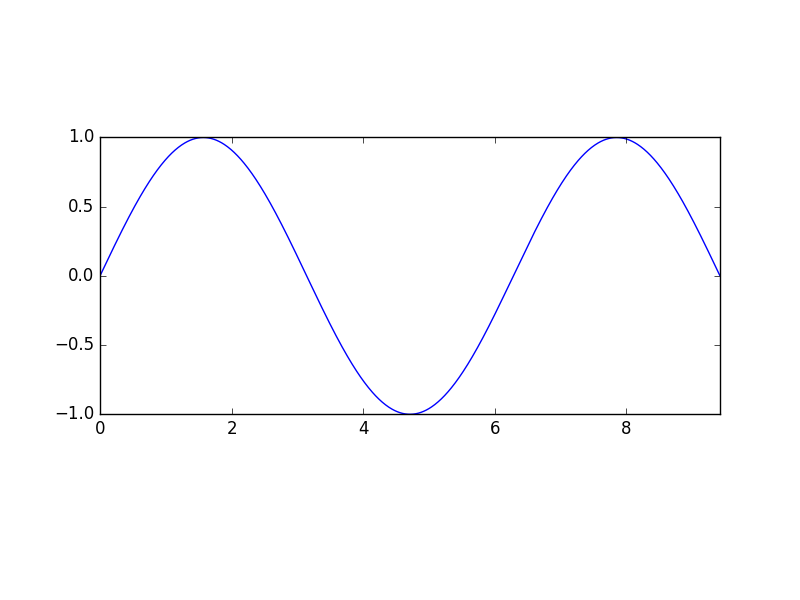
\includegraphics[scale=.35]{resultsCodigos/seno3}
				\captionof{figure}{Gráfico da função $y(x) = \sin(x)$}
			\end{minipage}%
			\begin{minipage}{.5\textwidth}
				\centering
				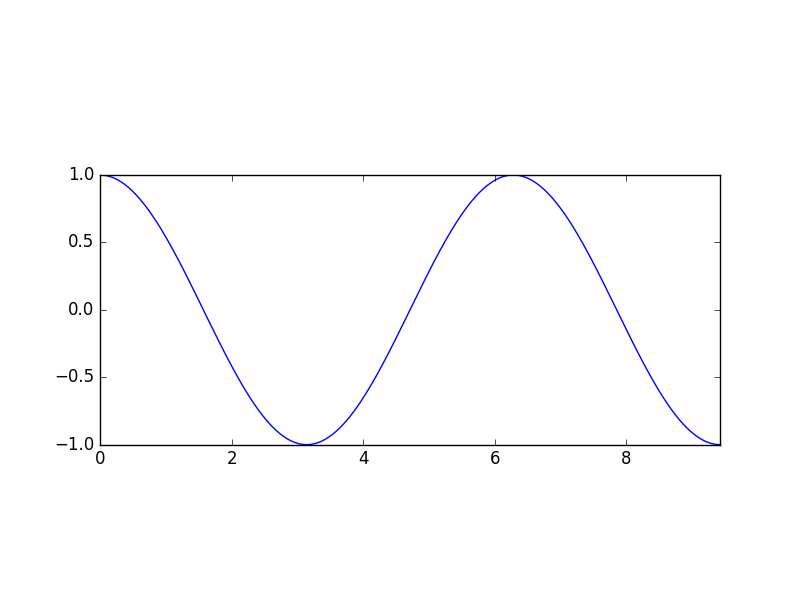
\includegraphics[scale=.35]{resultsCodigos/cosseno}
				\captionof{figure}{Gráfico da função $y(x) = \cos(x)$}
			\end{minipage}
		\end{figure}
		
		Dessa forma, pode-se entender o motivo do nome senoidal.
		
		\lstset{language=Python}
		\begin{lstlisting}
#Codigo para plotagem do seno

import numpy as np
import matplotlib.pyplot as plt

pi = 3.14159265359
xvals = np.arange(0, 3*pi, 0.01)
yvals = np.sin(xvals)
plt.plot(xvals, yvals)
plt.axis([0, 3*pi, -1, 1])
plt.show()
		\end{lstlisting}
		
		\begin{lstlisting}
#Codigo para plotagem do cosseno

import numpy as np
import matplotlib.pyplot as plt

pi = 3.14159265359
xvals = np.arange(0, 3*pi, 0.01)
yvals = np.cos(xvals)
plt.plot(xvals, yvals)
plt.axis([0, 3*pi, -1, 1])
plt.show()
		\end{lstlisting}
		
	\section{A Equação Geral da Onda}
		O comportamento das ondas pode ser estudado através da equação geral da onda
		
		\begin{equation}
		    \frac{\partial^2 u}{\partial t^2} = \frac{1}{v}\frac{\partial^2 u}{\partial x^2}
		\end{equation}
		na qual, $v$ representa a velocidade de propagação da onda e $t$ representa o tempo. Essa equação foi obtida por meio da aplicação da segunda lei de Newton ao movimento dos elementos do meio em que a onda se propaga, como os elementos de uma fita, por exemplo. Essa equação é uma equação diferencial geral parcial (a ser estudada mais a fundo no capítulo \ref{cap:EDPs}), o que indica que existem taxas que se relacionam no fenômeno.
	
	\section{Algumas Aplicações do Estudo de Ondas}
		Como dito anteriormente, o estudo do fenômeno físico das ondas possibilita um melhor bem-estar para a humanidade. Ele pode ser utilizado, por exemplo, nas áreas:
		\begin{itemize}
			\item\textbf{Acústica: }o estudo apropriado das ondas sonoras facilita o alcance do som de uma orquestra até a sua plateia, por exemplo, contribuindo para as Artes e Cultura;
			
			\item\textbf{Sísmica: }o estudo sobre as ondas sísmicas podem facilitar a previsão de terremotos e a evolução da tecnologia de prédios resistentes a tremores de alta intensidade;
			
			\item\textbf{Estruturas: }pontes usadas em grandes estradas, por exemplo, costumam estar em contato constante com ondas marítimas ou fluviais, além do próprio vento. Se os cálculos dos engenheiros responsáveis pela construção das mesmas não assegurar a estabilidade da ponte, a mesma pode ruir pelo fenômeno da ressonância ou pelo impacto constante das ondas.
			
		\end{itemize}

